\hypertarget{constantes_8hpp}{
\section{/home/arnaud/programmation/sfml/sfgui/constantes.hpp File Reference}
\label{constantes_8hpp}\index{/home/arnaud/programmation/sfml/sfgui/constantes.hpp@{/home/arnaud/programmation/sfml/sfgui/constantes.hpp}}
}


This graph shows which files directly or indirectly include this file:\nopagebreak
\begin{figure}[H]
\begin{center}
\leavevmode
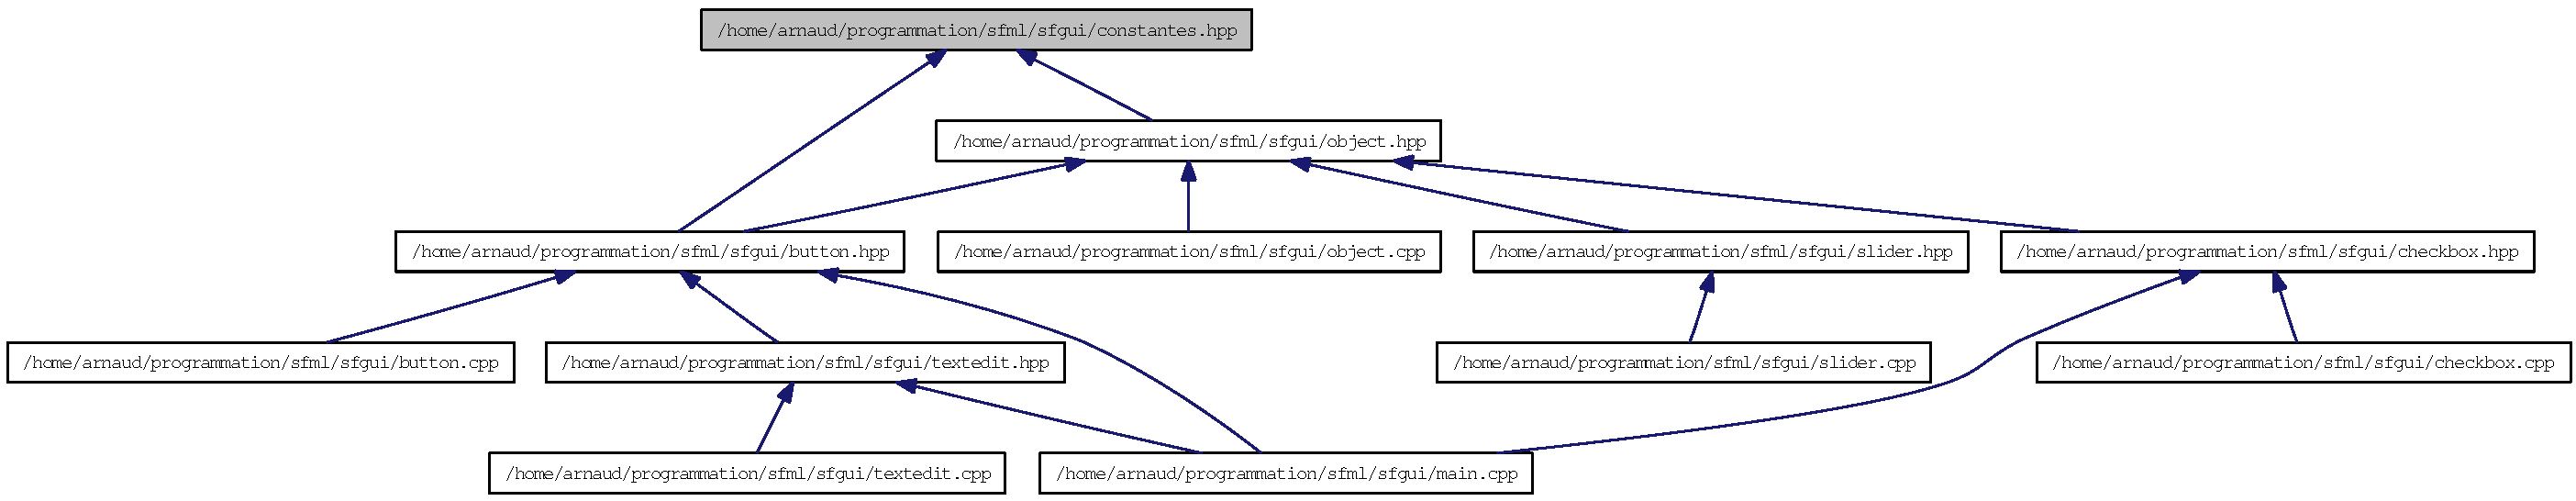
\includegraphics[width=420pt]{constantes_8hpp__dep__incl}
\end{center}
\end{figure}
\subsection*{Namespaces}
\begin{CompactItemize}
\item 
namespace \hyperlink{namespacesfgui}{sfgui}
\end{CompactItemize}
\subsection*{Enumerations}
\begin{CompactItemize}
\item 
enum \{ \hyperlink{namespacesfgui_ed969f0aaa542b462035e828757f431328ce9405120beac8fae51bc232aeabec}{sfgui::Left}, 
\hyperlink{namespacesfgui_ed969f0aaa542b462035e828757f4313d4fbbcf5a5a40412eeb0175f82c85b3f}{sfgui::Right}, 
\hyperlink{namespacesfgui_ed969f0aaa542b462035e828757f43130172869b534ad2378e28e388342699cc}{sfgui::Center}
 \}
\end{CompactItemize}


\subsection{Detailed Description}
\begin{Desc}
\item[Author:]TANGUY Arnaud $<$\href{mailto:arn.tanguy@gmail.com}{\tt arn.tanguy@gmail.com}$>$ \end{Desc}
\begin{Desc}
\item[Date:]2009 \end{Desc}
\begin{Desc}
\item[Version:]0.1 \end{Desc}
